% !TeX root = ../praktikum.tex
% !TeX encoding = UTF-8
% !Tex spellcheck = de_DE


Anhand der aufgenommenen Messdaten des Versuchsteils zur Winkelabhängigkeit wurde nun die Abhängigkeit des Quanten-Hall-Effekts, sowie des Shubnikov-de Haas-Effekts vom Einfallswinkel des Magnetfeldes auf die Probe analysiert.
Dazu wurden in Abbildung \ref{fig:winkel_ausw} die Magnetfeldwerte der Minima in Abhängigkeit des Winkels zur Probennormalen aufgetragen. 
Ein hier angegebener Winkel von $300^\circ$ entspricht einer Auslenkung aus der Normalen der Probe zum Magnetfeld von $70^\circ$, da die Zahlen auf der Winkelscheibe übernommen wurden. Ein angegebener Winkel von $360^\circ$ entspräche also einer tatsächlichen Auslenkung von $10^\circ$. 
In der Graphik wurden die Werte eines bestimmten Minimas bei unterschiedlichen Winkeleinstellungen gegen das reziproke Magnetfeld $\nicefrac{1}{B}$ aufgetragen. Zudem wurden hier die Positionen zweier verschiedener Minima (Minimum 1 in rot, Minimum 2 in blau dargestellt) verglichen und um in einem Graphen vergleichbar dargestellt zu werden, auf den jeweils Maximalen Wert zu 1 normiert. 
Zwischen den Einstellungen 370 bis $320^{\circ}$ verläuft die Kurve Cosinusförmig. Bei Werten weiter links auf der x-Achse, welche hier einer größeren Auslenkung aus der Null-Position entsprechen, weicht die Kurve immer mehr von dieser Form ab. Für die Winkelabhängigkeit der beiden betrachteten Effekte wird theoretisch eine Cosinusfunktion erwartet, da bei einem Winkel von $0^{\circ}$ das effektive Magnetfeld am stärksten und bei einem Winkel von $90^{\circ}$ zur Probenfläche gleich Null ist. Ausgedrückt wird diese Beziehung durch das Skalarprodukt

\begin{equation}
\vec{B}=\abs{\vec{B}} \cdot cos(\alpha)
\label{eq:winkelabh_skalarprodukt}
\end{equation}

Mit dem Winkel $\alpha$ zwischen Magnetfeldlinien und Probennormalen. Das Abweichen der Kurve vom Verlauf einer Cosinusfunktion ab einem Winkelwert von $320^{\circ}$, also einer Auslenkung $>50^{\circ}$, wird hier auf statistische Fehler zurückgeführt. Der Fehler des Probenwinkels wird auf einen Wert von $\nicefrac{+}{-} 3 $ Grad geschätzt und folgt ebenso wie der Fehler des reziproken Magnetfeldes, welcher pauschal auf $\nicefrac{+}{-} \unit[0,01]{T}0,01$ geschätzt wird, aus Ablesefehlern. 
Aufgrund des reziproken Auftragens des Magnetfeldes auf der y-Achse sind deren einzelne Fehler der Messpunkte um einen Faktor von bis zu $10^{-5}$ kleiner als die y-Werte selbst und wurden daher nicht im Graphen dargestellt.
Verglichen mit dem Graphen liegen die theoretisch erwarteten Werte etwa um $+3$ Grad in Auslenkungsrichtung verschoben, das heißt, es liegt auch für die Werte geringerer Auslenkung ein leichtes Offset vor. Dies verdeutlichen die beiden Kurven der Funktionen $cos(\nu)$ und $cos(\nu-3^{\circ})$ im selben Graphen. Es ist gut zu erkennen, dass die Kurve der Funktion $cos(\nu-3^{\circ})$ näher an den aus den Messdaten erhaltenen Werten liegt. 

\begin{figure}[h]
	\centering
	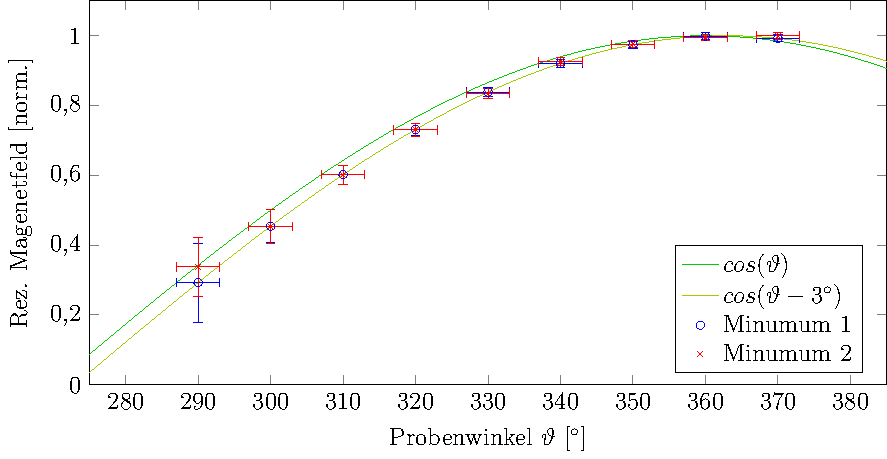
\includegraphics[scale=1]{graphs/winkel/auswertung.pdf}
	\caption[]{
		}
		\label{fig:winkel_ausw}
\end{figure}

Dies lässt vermuten, dass die Winkelscheibe, an welcher die relative Position der Probennormalen zu den Magnetfeldlinien abgelesen wurde, um 3 Grad aus der Nullposition ausgelenkt angebracht ist. 
Die hier dargestellte Abhängigkeit zeigt dennoch deutlich, dass für zunehmende Auslenkung aus der Nullposition höhere Magnetfelder, also kleinere Werte für $\frac{1}{B}$ notwendig sind, um für die SDH-Oszillation Minima zu erzeugen und es kann angenommen werden, dass diese bei einer Auslenkung von 90 Grad vollständig verschwinden. 

